\chapter{Cálculo en Variedades}\label{Capítulo: Cálculo en Variedades}
En este capítulo describiremos algunos conceptos básicos que eventualmente nos ayudarán a entender qué son las métricas, qué es una métrica Riemanniana y lo que son las variedades Riemannianas.

\section{Espacios Tangentes}
\subsection{Espacios Tangente en $\R^n$}


Los primeros conceptos que estudiaremos serán los espacios y fibrados tangentes. Existen varias definiciones equivalentes para lo que es un espacio tangente; nosotros procederemos a definirlo a partir de lo que llamaremos derivaciones, este enfoque tiene algunas ventajas algebraicas y se puede justificar con conceptos conocidos de cálculo multivariable. Comenzaremos contextualizando lo que queremos decir por espacio tangente en $\R^n$ y después generalizaremos la idea a variedades suaves.

Antes de comenzar necesitamos hacer la siguiente aclaración sobre la notación que utilizaremos, si consideramos un punto $p$ en $\R^n$ y queremos describir explícitamente sus coordenadas, esto lo haremos escribiendo entre paréntesis, $p = (p_1, \ldots, p_n)$; si en cambio consideramos un vector $v$ en $\R^n$, este puede ser representado por una matriz $n \times 1$, sin embargo, por conveniencia escribiremos $v = \begin{bmatrix} v_1 & \cdots & v_n \end{bmatrix}$, sin perder de vista que en realidad estamos hablando de la transpuesta de esta matriz.

\begin{definition}[Vectores y Espacios Tangentes en $\R^n$]\label{Definición: Espacio Tangente en Rn}
	Sea $a$ un punto en $\R^n$, definiremos el \it{espacio tangente a $\R^n$ en el punto $a$}, denotado por $T_a(\R^n)$, como el conjunto:
	\[ \{a\} \times \R^n = \{(a,v): v \in \R^n\}. \]
	Un \it{vector tangente} a $\R^n$ es un elemento de $T_a(\R^n)$ para algún $a \in \R^n$. Denotaremos a un vector tangente $(a,v)$ particular como $v_a$ o $v|_a$ o simplemente $v$ para abreviar.
\end{definition}

En palabras más simples, lo que esta definición nos está diciendo es que el espacio tangente a $\R^n$ en algún punto $a$ es la colección de todos los vectores en $\R^n$ con origen en $a$.

Una de las propiedades más importantes del conjunto $T_a(\R^n)$ es que es un espacio vectorial bajo las operaciones
\[ v_a + w_a = (v + w)_{a}, \quad c(v)_{a} = (cv)_{a}. \]
Por ser un espacio vectorial tendrá una base, no es difícil ver que si $\{e_i\}_{i=1}^n$ son los vectores de la base canónica para $\R^n$, entonces $\{e_i|_{a}\}_{i=1}^n = \{(a,e_i)\}_{i=1}^n$ será una base para $T_a(\R^n)$, al tener $n$ vectores básicos; llamamos a esta base la base estándar. $T_a(\R^n)$ será un espacio vectorial $n-$dimensional y por lo tanto será isomorfo a $\R^n$, de hecho $T_a(\R^n)$ es una copia de $\R^n$.

\begin{center}
	\begin{figure}[h]
		\centering
		\begin{subfigure}{0.30\textwidth}
			\centering
			\begin{tikzpicture}
\draw[thick,->] (-0.5,0) -- (5,0) node[anchor=west]{$x$};
\draw[thick,->] (0,-0.5) -- (0,5) node[anchor=south]{$y$};

\draw (0.5,0.5) rectangle (4,4);
\node at (4.5,4.5) {$T_a(\R^n)$};

\draw[thick,->] (1,1.5) -- (3.5,1.5);
\draw[thick,->] (1.5,1) -- (1.5,3.5);
\filldraw (1.5,1.5) circle (0.1);
\node at (1,1) {$a$};
\draw[thick, ->] (1.5,1.5) -- (3,2.75);
  \node at (3.25,2.5) {$v_a$};
\end{tikzpicture}


		\end{subfigure}
		\hspace{60pt}
		\begin{subfigure}{0.30\textwidth}
			\centering
			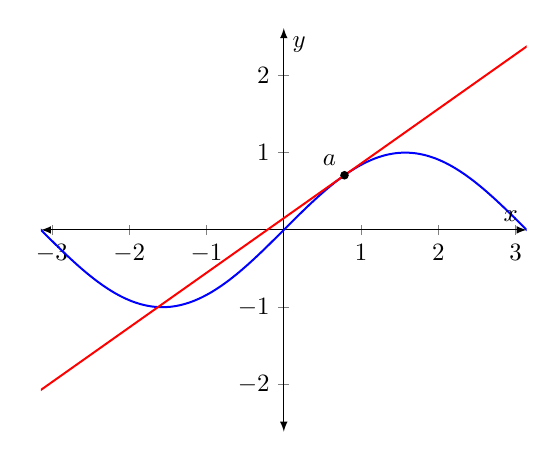
\begin{tikzpicture}[scale=0.90]
	\begin{axis}[
			% grid=both,
			xmin=-pi,
			xmax=pi,
			ymin=-1.6,
			ymax=1.6,
			axis lines=middle,
			xlabel = $x$,
			ylabel = $y$,
			axis line style={latex-latex},
      axis equal,
		]

		\addplot[
			samples=200,
			domain=-4*pi:4*pi,
			color=blue,
			thick,
			smooth,
		]
		{sin(deg(x))};

		\addplot[
			domain=-5:5,
			color=red,
      thick,
		]{( (sqrt(2) / 2) * (x - (pi/4)) ) +  (sqrt(2) / 2)};

		\addplot+[
			mark options={black},
      mark size=1.5pt,
		] coordinates {(0.785398,0.707106)} node [black, left=6pt, above=0.5pt] {$a$};
	\end{axis}
\end{tikzpicture}


		\end{subfigure}
		\\[20pt]
		\begin{subfigure}{0.30\textwidth}
			\centering
			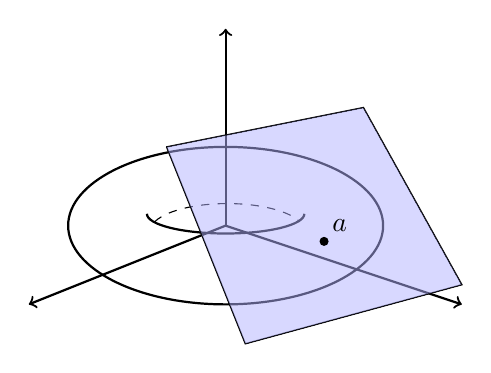
\begin{tikzpicture}

	% Ejes R3
	\draw [thick,->] (0,0) -- (0,2.5);
	\draw [thick,->] (0,0) -- (3,-1);
	\draw [thick,->] (0,0) -- (-2.5,-1);

	% Toro
	\draw [thick] (0,0) ellipse  (2 and 1);
	\draw [thick] (-1.0,0.15) arc (0:-180:-1.0 and 0.25);
  \draw [dashed] (-0.90,0.05) arc (20:160:-0.98 and 0.35);

  % Plano tangente
  \draw [line width=0.5] (-0.75,1) -- (1.75,1.5) -- (3,-0.75) -- (0.25,-1.5) -- (-0.75,1);
  \draw [fill=blue!30!white,opacity=0.5, line width=0] (-0.75,1) -- (1.75,1.5) -- (3,-0.75) -- (0.25,-1.5) -- (-0.75,1);

  % Punto $a$
	\filldraw (1.25,-0.2) circle (0.05);
	\node at (1.45,0) {$a$};
\end{tikzpicture}

		\end{subfigure}
		\hspace{60pt}
		\begin{subfigure}{0.30\textwidth}
			\centering
			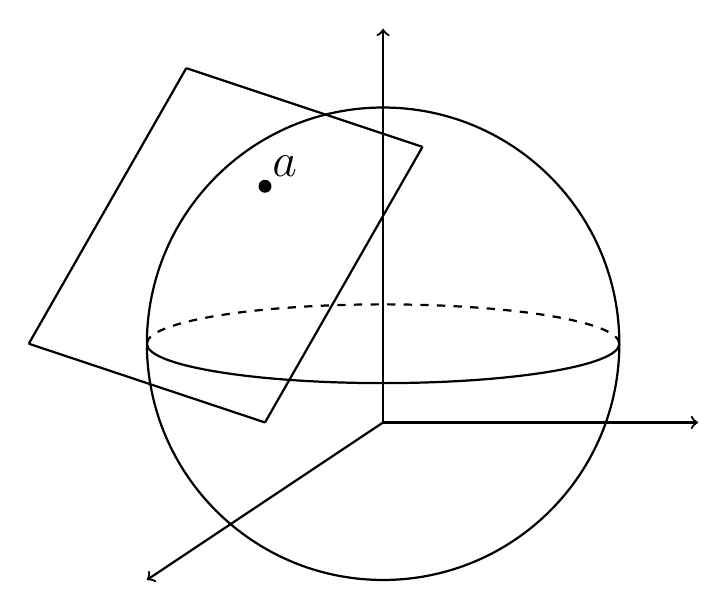
\begin{tikzpicture}
  % Esfera
  \draw [thick] (3,0) arc (0:180:3 and -0.5);
  \draw [thick, dashed] (-3,0) arc (180:0:3 and 0.5);
  \draw [thick] (0,0) circle (3);

  % Ejes R3
  \draw [thick,->] (0,-1) -- (0,4);
  \draw [thick,->] (0,-1) -- (4,-1);
  \draw [thick,->] (0,-1) -- (-3,-3);


  % Rectángulo (Espacio Tangente)
  \filldraw (-1.5,2) circle (0.075);
  \node[font=\fontsize{18pt}{18pt}] at (-1.25,2.25) {$a$};
  \draw [thick] (-2.5,3.5) -- (0.5,2.5);
  \draw [thick] (-2.5,3.5) -- (-4.5,0);
  \draw [thick] (-4.5,0) -- (-1.5,-1);
  \draw [thick] (0.5,2.5) -- (-1.5,-1);
\end{tikzpicture}

		\end{subfigure}
		\caption{Visualización de espacios tangentes a diferentes variedades.}
	\end{figure}
\end{center}

Si en $\R^n$ consideramos un punto $a = (a_1, \dots, a_n)$ y un vector $v = \begin{bmatrix} v_1 \dots v_n \end{bmatrix}$, podemos dar la siguiente parametrización para la recta que pasa por $a$ con en la dirección de $v$:
\[ \gamma(t) = (a_1 + tv_1, \dots, a_n + tv_n). \]

\begin{definition}[Derivada Direccional]\label{Definción: Derivada Direccional}
	Sea $f: \R^n \to \R$ una función suave definida en una vecindad de un punto $a$ y $v \in T_a(\R^n)$, la \it{derivada direccional} de $f$ en $a$ en la dirección de $v$ se define como:
	\[ D_v f = \left. \frac{d}{dt} \right|_{t=0} f(\gamma(t)). \]
\end{definition}

Por la regla de la cadena podemos escribir la derivada direccional como:
\[
	D_v f
	= \sum_{i=1}^{n} \frac{d \gamma_i(0)}{dt} \frac{\partial f}{\partial x_i} (a)
	= \sum_{i=1}^n v_i \frac{\partial f}{\partial x_i} (a).
\]

En este sentido, cada vector tangente $v_a \in T_a(\R^n)$ nos define un mapeo $D_v: C^{\infty}(\R^n) \to \R$ que nos da la derivada direccional de funciones suaves en un punto $a$ en la dirección de $v$. Dado que evaluamos la derivada direccional en el punto $a$, $D_v(f)$ será un número real.

Sabemos de cálculo que la derivada direccional es un operador lineal y además cumple la regla de Leibniz, esto es, si $f$ y $g$ son funciones suaves definidas en una vecindad de $a$, $c$ es una constante y $v$ es un vector tangente, entonces:

\begin{itemize}
	\item $D_v(cf) = c D_v(f)$.
	\item $D_v(f+g) = D_v(f) + D_v(g)$.
	\item $D_v(fg) = f(a) D_v(g) + g(a) D_v(f)$.
\end{itemize}

Basados en esta propiedad daremos la siguiente definición

\begin{definition}[Derivación en un punto]\label{Definición: Derivación en un punto de Rn}
	Sea $a$ un punto en $\R^n$ y $\omega: C^{\infty}(\R^n) \to \R$, diremos que $\omega$ es una \it{derivación en $a$} si es lineal y cumple la regla de Leibniz, i.e., si $f$ y $g$ son funciones suaves definidas en una vecindad de $a$, $c$ una constante
	\begin{itemize}
		\item $\omega(cf) = c \omega(f)$.
		\item $\omega(f+g) = \omega(f) + \omega(g)$.
		\item $\omega(fg) = f(a) \omega(g) + g(a) \omega(f)$.
	\end{itemize}
	Denotaremos al conjunto de todas las derivaciones de $C^{\infty}(\R^n)$ en el punto $a$ como $\D_a(\R^n)$.
\end{definition}

De modo similar a $T_a(\R^n)$, $\D_a(\R^n)$ es un espacio vectorial bajo las operaciones
\[ (\omega_1 + \omega_2)(f) = \omega_1(f) + \omega_2(f), \quad (c\omega)(f) = c(\omega(f)) \]
y más aún, con ayuda del siguiente lema probaremos que $\D_a(\R^n)$ es isomorfo a $T_a(\R^n)$.

\begin{lemma}\label{Lemma: Propiedades de las Derivaciones}
	Sea $a \in \R^n$ un punto, $\omega \in \D_a(\R^n)$ y $f,g \in C^{\infty}(\R^n)$. Entonces:
	\begin{itemize}
		\item Si $f$ es una función constante, $\omega(f) = 0$.
		\item Si $f(a) = g(a) = 0$, entonces $\omega(fg) = 0$.
	\end{itemize}
\end{lemma}

\begin{proof}
	\begin{itemize}
		\item Basta probar el caso en que $f \equiv 1$, el caso general se tiene por la linealidad de $\omega$. Si $f \equiv 1$, entonces:
		      \begin{align*}
			      \omega(f) & = \omega(f \cdot f)             \\
			                & = f(a)\omega(f) + f(a)\omega(f) \\
			                & = 2\omega(f)
		      \end{align*}
		      Esto implica que $\omega(f) = 0$.
		\item Si $f(a) = g(a) = 0$, entonces por definición de derivación se tiene que:
		      \[ \omega(fg)= f(a)\omega(g) + g(a)\omega(f) = 0  \]
	\end{itemize}
\end{proof}

Dado que las derivadas direccionales en un punto $a$ son lineales y cumplen la regla de Leibniz, estas serán derivaciones en $a$ por definición. Esto implica que existe un operador lineal $\phi$ entre $T_a(\R^n)$ y $\D_a(\R^n)$ tal que:
\begin{align*}
	\phi: T_a(\R^n) & \to \D_a(\R^n) \\
	v               & \mapsto D_v =
	\left. \sum_{i=1}^{n} v_i \frac{\partial}{\partial x_i} \right|_a
\end{align*}

\begin{theorem}\label{Teorema: Isomorfismo entre Espacio Tangente y Espacio de Derivaciones}
	El mapa $\phi: T_a(\R^n) \to \D_a(\R^n)$ es un isomorfismo de espacios vectoriales.
\end{theorem}

\begin{proof}
	La linealidad se tiene trivialmente, dado que como acabamos de mencionar, las derivadas direccionales en un punto lo son. Debemos mostrar que $\phi$ es inyectiva y sobreyectiva. Para mostrar que $\phi$ es una función inyectiva, mostraremos que su kernel es cero.

	Tomemos un vector $v \in T_a(\R^n)$ tal que $D_v \equiv 0$. Si tomamos la función $f: \R^n \to \R$ como la $j-$ésima función coordenada $x_j: \R^n \to \R$ tendremos que
	\begin{align*}
		0 = D_v(x_j) & = \left. \sum_{i=1}^{n} v_i \frac{\partial}{\partial x_i} \right|_{a} x_i \\
		             & = \sum_{i=1}^{n} v_i \delta_i^j = v_j
	\end{align*}

	Dado que esto se cumple para cada $j$, se sigue que $v \equiv 0$, y por lo tanto $\phi$ es una función inyectiva.

	Para mostrar que $\phi$ es una función sobreyectiva supongamos que $\omega \in \D_a(\R^n)$, esto es, $\omega$ es una derivación en el punto $a = (a_1, \dots, a_n)$, y sea $v = \begin{bmatrix} v_1 & \cdots & v_n \end{bmatrix}$ un vector en $T_a(\R^n)$. Podemos representar a $v$ en la base estándar de $\R^n$ como $v = \sum_{i=1}^{n} v_i e_i$, si definimos a $v$ de modo que cada $v_i$ sea el número real dado por la relación $v_i = \omega(x_i)$ tendremos que $\omega = D_v$.

	En efecto, si $f: \R^n \to \R$ es una función suave definida en una vecindad de $a$, entonces, por el Teorema de Taylor tenemos que existen funciones suaves definidas en una vecindad de $a$ tal que:
  \begin{align*}
    f(x) = f(a) 
    &+ \sum_{i=1}^{n} \frac{\partial f}{\partial x_i} (a) (x_i - a_i) \\
    &+ \sum_{i=1}^{n} \sum_{j=1}^{n} (x_i - a_i)(x_j - a_j) \int_{0}^{1} (1-t) \frac{\partial^2 f}{\partial x_i \partial x_j} (a + t(x - a))
  \end{align*}

	Notemos lo siguiente, $f(a)$ es una constante y el último término es la suma del producto de dos funciones suaves, $(x_i - a_i)$ y $(x_j - a_j)$ por la integral; ambos términos se anulan en $x = a$, por lo que, por el lema anterior, al aplicar $\omega$ a la serie de Taylor el primer y el último término se anularan, obteniendo:
	\begin{align*}
		\omega(f) & = \omega(\sum_{i=1}^{n} \frac{\partial f}{\partial x_i} (a )(x_i - a_i))        \\
		          & = \sum_{i=1}^{n} \frac{\partial f}{\partial x_i} (a)(\omega(x_i) - \omega(a_i)) \\
		          & = \sum_{i=1}^{n} \frac{\partial f}{\partial x_i}(a) v_i = D_v f
	\end{align*}
	Por lo tanto $\phi$ es una función lineal, inyectiva y sobreyectiva entre espacios vectoriales, esto es, $\phi$ es un isomorfismo entre $T_a(\R^n)$ y $\D_a(\R^n)$.
\end{proof}

Este teorema nos permite identificar el espacio tangente en un punto con el espacio de de derivaciones en el mismo punto, lo cual denotamos por $T_a(\R^n) \simeq \D_a(\R^n)$, además, la existencia de este isomorfismo tiene como consecuencia el siguiente corolario.

\begin{corollary}\label{Corolario: Base de TpRn}
	Para cada $a \in \R^n$, las $n$ derivadas parciales
	\[
		\left. \frac{\partial }{\partial x_1} \right|_{a}, \dots, \left. \frac{\partial }{\partial x_n} \right|_{a},
	\]
	forman una base para el espacio tangente $T_a(\R^n)$.
\end{corollary}

Esta identificación nos permite escribir a los vectores de $\R^n$, $v = \begin{bmatrix} v_1 & \cdots & v_n \end{bmatrix}$ como una combinación lineal de la forma:
\[ 	v = \left. \sum_{i = 1}^{n} v_i \frac{\partial}{\partial x_i} \right|_{a}.\]
